\section{Reflection on Learning} \label{sec:reflection}

Throughout the course of the final year project, I have gained invaluable experience and insight into the challenges and rewards of research and development. The process has provided me with opportunities to refine my technical skills and enhance my understanding of DRL. However, there have also been areas where I could have improved my approach, which I would like to address in this reflection on learning.

\subsection{Inadequate logging practices}

One challenge I faced during the project was reproducing issues that had previously occurred. This was mainly due to insufficient logging and documentation of my work as I progressed. Although I used version control system to maintain the development of the software, I realised the importance of maintaining a detailed record of the steps taken, the hyperparameters used, and the outcomes observed, as it would have allowed me to efficiently identify and address problems, especially for experiments.

In future projects, I will log progresses in daily basis to ensure that any issues encountered can be easily reproduced and resolved. Figure \ref{fig:daliy-log} is a typical example.

\begin{figure}[htbp]
   \centering
   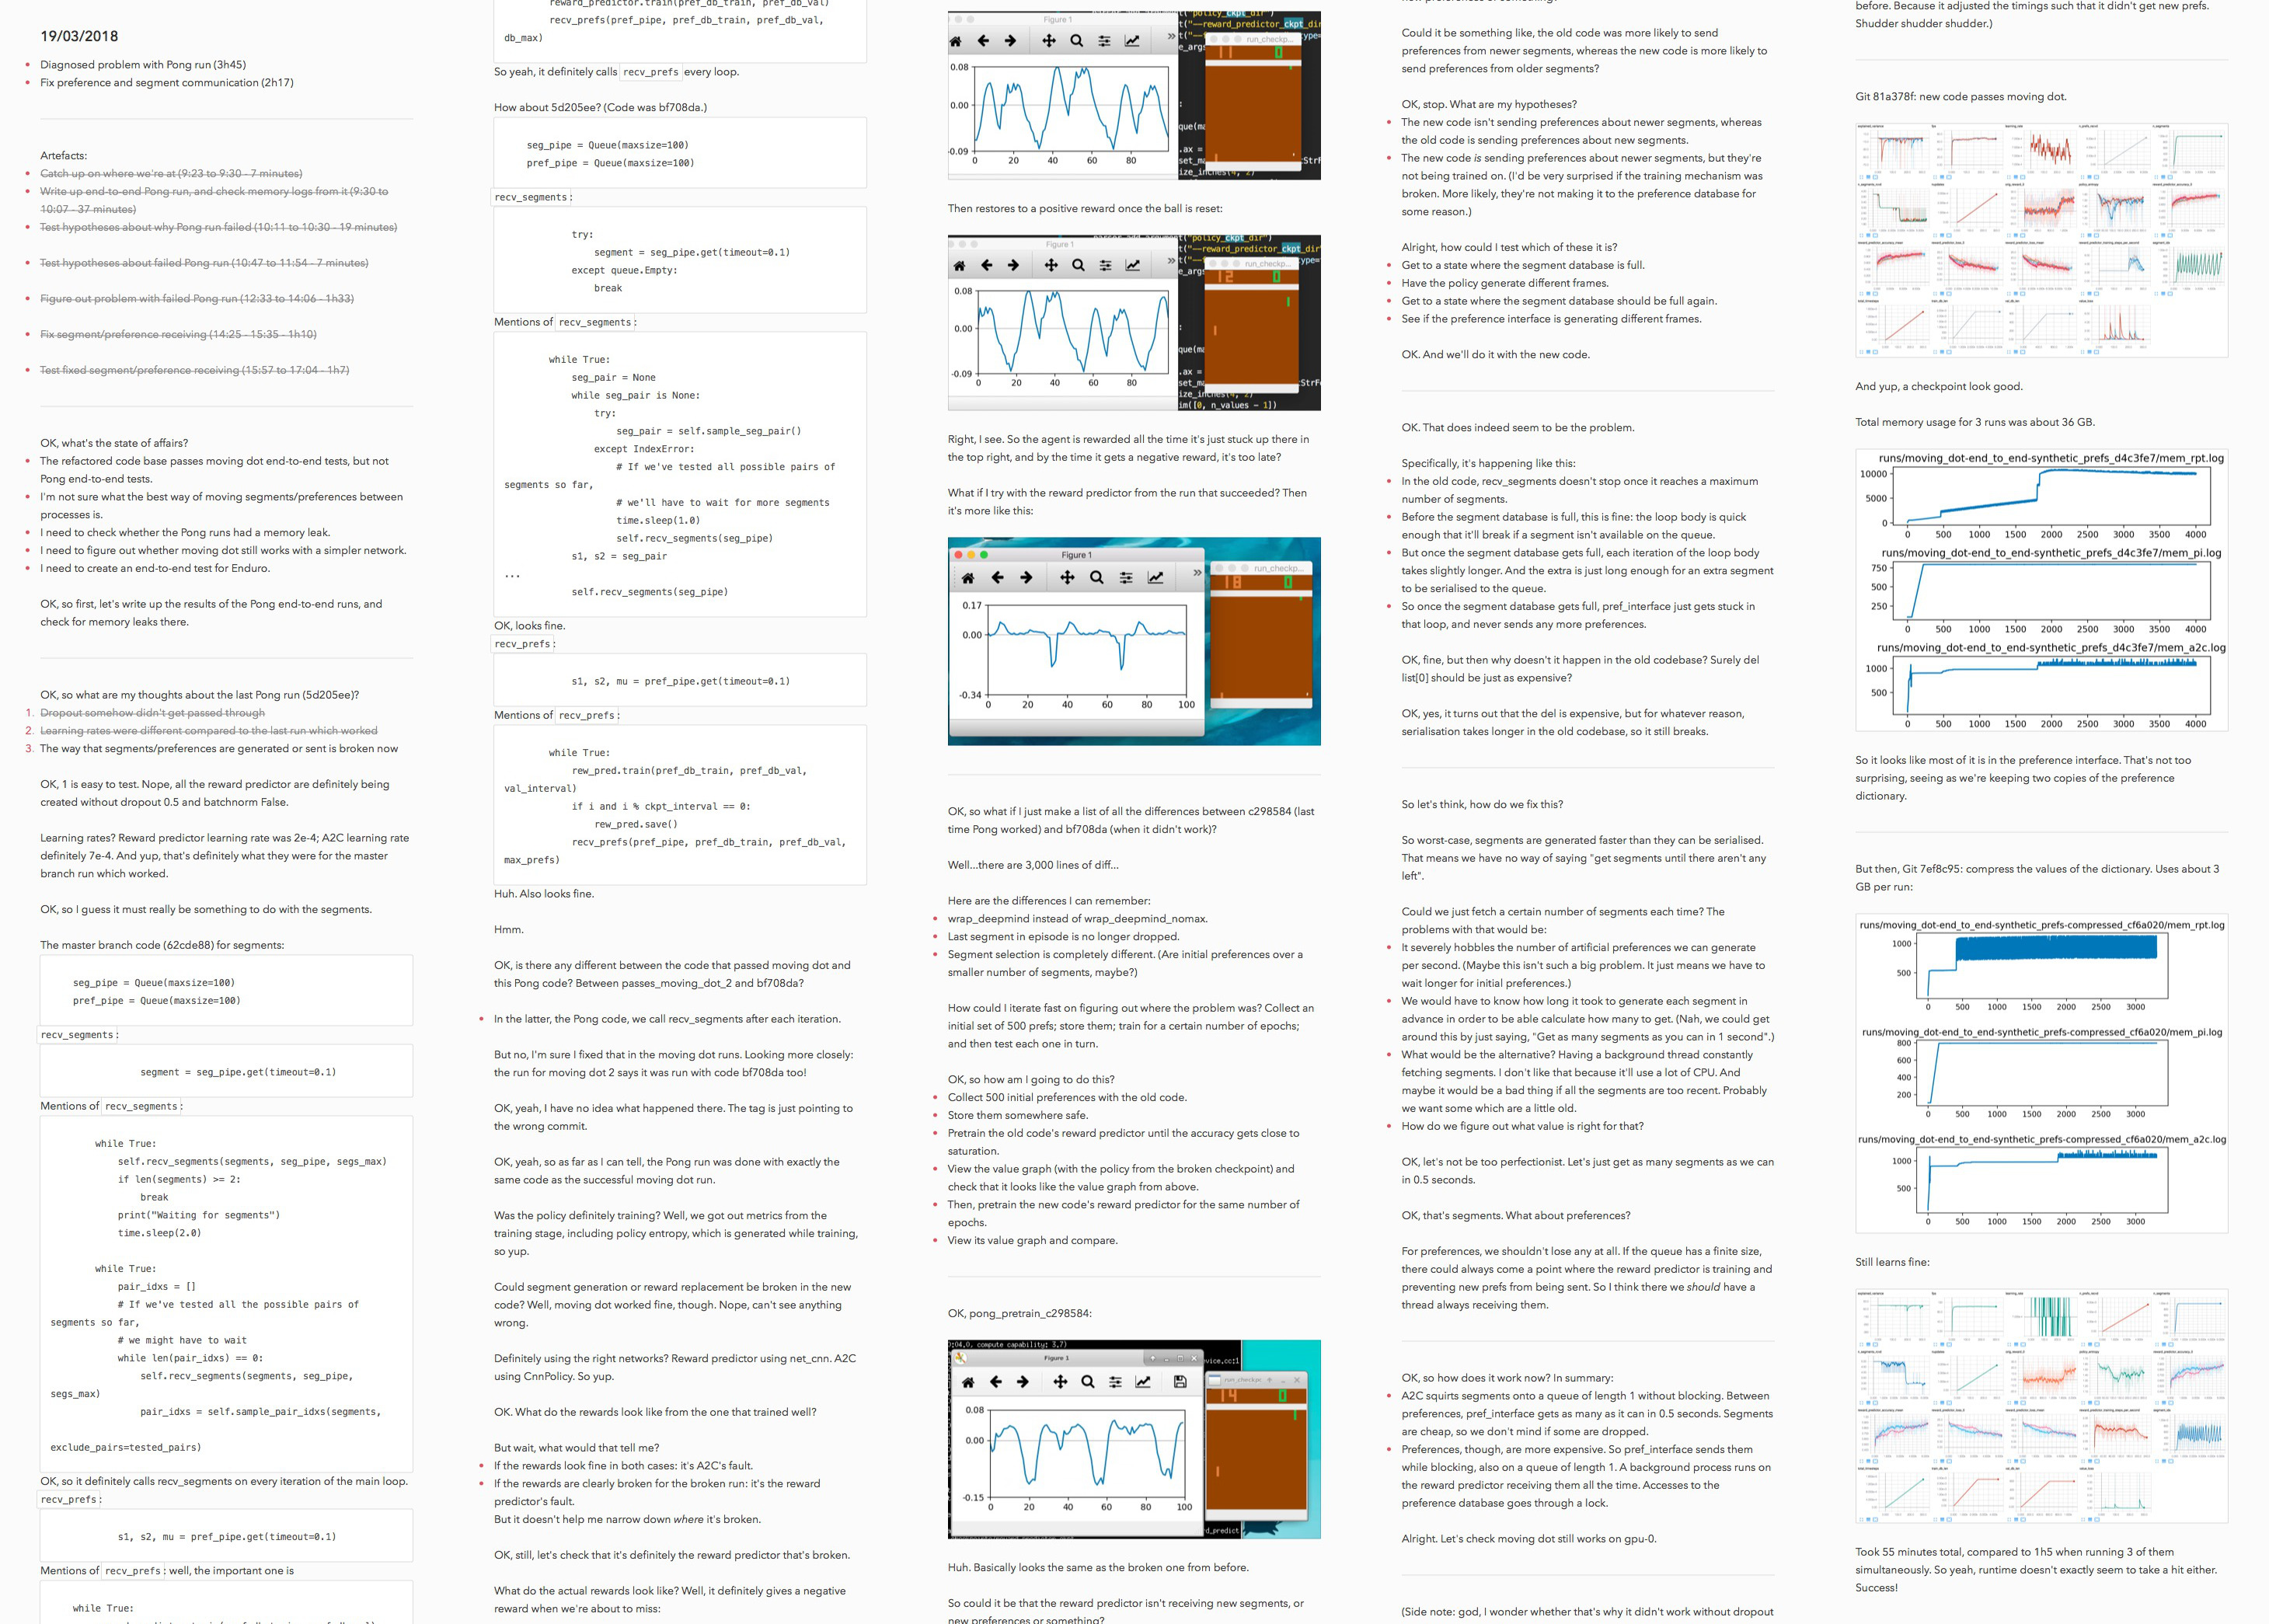
\includegraphics[width=0.9\textwidth]{a-rl-daliy-log.jpg}
   \caption{A typical daily log \cite{ref:reproducing-drl}.}
   \label{fig:daliy-log}
\end{figure}

\subsection{Comprehensive specification report}

With hindsight, I should have invested more time and effort into producing a thorough and detailed specification report. This would have not only provided a more solid foundation for my project but also streamlined the process of preparing the final report. Much of the information and content from the specification report could have been directly incorporated into the final document, saving time and effort in the long run.

For future endeavours, I will focus on creating a comprehensive specification report, as it will contribute significantly to the overall success of my projects.

\subsection{Advance report drafting}

I learned the importance of writing the report earlier. Due to time constraints and other obligations, I found myself rushing to complete the final report towards the end of the project. This made the process stressful and challenging and resulted in a greater likelihood of errors or omissions in the final document. I realised that starting early and allocating more time to report writing could have prevented this situation.

Therefore, in future projects, I will set aside more time to work on reports to ensure that I am not rushing to complete them towards the end.

\subsection{Foundational knowledge acquisition}

During the course of my project, I devoted significant time to reading research papers in order to gain a deeper understanding of the subject matter. However, I discovered that this approach did not provide me with a solid foundation in the fundamental concepts and principles of the field. In retrospect, I should have allocated more time to studying textbooks and other resources that offered a comprehensive overview of the basics before diving into the specialised research papers.

For future projects, I will adopt a more balanced approach by first focusing on mastering the foundational knowledge through textbooks, lectures, and online courses. This will ensure that I have a strong grasp of the essential concepts and can better contextualise the findings and insights presented in research papers.
